\section{Critical Points and Extrema: Further Topics}\label{sec:multi_extreme_further}

\noindent\textbf{\large Constrained Optimization and Lagrange Multipliers}\\

Let us continue our discussion of constrained optimization begun in Section \ref{sec:multi_extreme_values}. Theorem \ref{thm:extreme_val3} tells us that the Extreme Value Theorem extends to functions of two variables; in fact, this is true for a function of any number of variables: if a real-valued function $f$ is continuous on a closed, bounded subset of $\mathbb{R}^n$, then it is guaranteed to have an absolute maximum and minimum.

However, as the number of variables increases, the job of finding these absolute extrema becomes more and more complicated. We saw one approach in Section \ref{sec:multi_extreme_values}: given a continuous function on a closed, bounded region $D$, we first consider critical values on the interior of $D$. We then restrict our function $f$ to points on the boundary of $D$, and attempt to reduce the problem to optimization in one variable.

In many cases, this approach is best accomplished by parametrizing the boundary. We learned how to define parametric curves in the plane in Section \ref{sec:param_eqs}.\\

\example{ex_optimize_param_bound}{Constrained optimization by parametrization}{
Find the absolute maximum and minimum values of $f(x,y) = x^2-8x-3y^2$ on the disc $x^2+y^2\leq 4$.}
{
First, we check for critical points: We have
\[
\nabla f(x,y) = \la 2x-8,-6y\ra,
\]
which vanishes when $(x,y) = (4,0)$. This critical point is outside our region, so we do not consider it.

Next, we look for extreme values on the boundary. The boundary of our region is the circle $x^2+y^2=4$, which we can parametrize using $x=2\cos t$, $y=2\sin t$, for $t\in [0,2\pi]$. For $(x,y)$ on the boundary, we have
\[
f(x,y) = x^2-8x-3y^2 = 4\cos^2t-16\cos t-12\sin^2t = h(t),
\]
a function of one variable, with domain $[0,2\pi]$. We learned how to find the extreme values of such a function way back in Calculus I: see Section \ref{sec:extreme_values}. We have $h(0)=h(2\pi)=-12$, and
\[
h'(t) = -8\cos t\sin t+16\sin t-24\sin t\cos t = 16\sin t (1-2\cos t).
\]
Thus, $h'(t)=0$ if $\sin t = 0$ ($t=0,\pi,2\pi$) or $\cos =\frac12$ ($t=\pi/3, 5\pi/3$). We have already checked that $h(0)=h(2\pi)=-12$, so we check the remaining points:
\begin{align*}
h(\pi) &= 4(-1)^2-16(-1) = 20\\
h(\pi/3)=h(5\pi/3) & = 4\left(\frac14\right)-16\left(\frac{1}{2}\right)-12\left(\frac34\right) = -16.
\end{align*}
We see that the absolute maximum is when $t=\pi$: $h(\pi) = f(-2,0)=20$, and the absolute minimum is $-16$, which occurs when $t=\pi/3$ and $t=5\pi/3$, corresponding to the points $(1,\sqrt{3})$ and $(1,-\sqrt{3})$, respectively. 
}\\

The above method works well, when it's straightforward to set up. The advantage is that it reduces the problem of optimization along the boundary to an optimization problem in one variable, which is something we mastered long ago.

One downside is that it is not always easy to come up with a parametrization for a curve. In the above example, the boundary $x^2+y^2=4$ is a \emph{level curve}: it's of the form $g(x,y)=c$. When we're trying to optimize subject to a constraint of this form, there is another approach, called the \sword{method of Lagrange multipliers}. \index{Lagrange multipliers}\index{optimization ! with Lagrange multipliers}.

Suppose we are trying to maximize a function $f(x,y)$ subject to a constrain $g(x,y)=c$. We could follow the approach given above: find a function $\vec{r}: [a,b]\to \mathbb{R}^2$ that parametrizes the curve $g(x,y)=c$. As we saw above, the maximum (or minimum) should occur at some point $t_0$ that is a critical number of $h(t)=f(\vec{r}(t))$; that is, such that 
\[
h'(t_0)=\nabla f(\vec{r}(t_0))\cdot \vrp (t_0) = 0.
\]
This tells us that the gradient $\nabla f$ should be orthogonal to the constraint curve $g(x,y)=c$ at the point $(x_0,y_0)=(x(t_0),y(t_0))$. But we know another gradient that is orthogonal to this curve: $\nabla g$! Recall from Theorem \ref{thm:gradient} that $\nabla g(x,y)$ is always orthogonal to the level curve $g(x,y)=c$ at points along the curve.

Let's sum up: the vectors $\nabla f(x_0,y_0)$ and $\nabla g(x_0,y_0)$ are both orthogonal to the vector $\vrp(t_0)$. We assume that $\nabla f(x_0,y_0)\neq \vec{0}$, since critical points of $f$ have already been checked. We also assume that $c$ is a \sword{regular value}\index{regular value} of $g$, meaning that there are no critical points of $g$ along the curve $g(x,y)=c$, so $\nabla g(x_0,y_0)\neq\vec{0}$ as well.

\mnote{.5}{\textbf{Note:} if $(x_0,y_0)$ is a critical point of a function $g$; that is, if $\nabla g(x_0,y_0)=\vec{0}$, and $g(x_0,y_0)=c$, we call the number $c$ a \sword{critical value}\index{critical value ! of a function of two variables} for $g$. Any number that is not a critical value is called a regular value. Often, if $c$ is a critical value, the level set defined by $g(x,y)=c$ is not a smooth curve, or even a curve at all. (For example, $g(x,y)=x^2+y^2$ has the critical point $(0,0)$, and critical value 0. The set of $(x,y)$ with $x^2+y^2=0$ is not a curve; it's a single point.)

Because of this, it's usually a safe assumption that when a level curve $g(x,y)=c$ is given, the value $c$ is a regular value.}

But the only way that two non-zero vectors in the plane can both be orthogonal to a third vector is if they're parallel! This means that there must be some scalar $\lambda$ such that
\[
\nabla f(x_0,y_0) = \lambda\nabla g(x_0,y_0).
\]
We have demonstrated the following:\\

\theorem{thm:lagrange_multipliers}{Location of constrained extrema}{
Let $f$ and $g$ be continuously differentiable functions of two variables, and suppose $c$ is a regular value for $g$. If the function $f$, when constrained to the level curve $g(x,y)=c$  has a local maximum or minimum value at a point $(x_0,y_0)$, then
\[
\nabla f(x_0,y_0) = \lambda \nabla g(x_0,y_0)
\]
for some scalar $\lambda$. 
}\\

Note that there are two possibilities: either $\lambda=0$, in which case $(x_0,y_0)$ is a critical point of $f$, or $\lambda\neq 0$, in which case the level curve of $f$ that passes through $(x_0,y_0)$ must be \emph{tangent} to the curve $g(x,y)=c$ at that point. Putting Theorem \ref{thm:lagrange_multipliers} to use is a matter of solving a system of equations.

\keyidea{idea:lagrange_multipliers}{Method of Lagrange Multipliers}{
To find the maximum and minimum values of a function $f$ of two variables subject to a constraint $g(x,y)=c$, we must find the simultaneous solutions to the following equations, where $\lambda$ is an unknown constant (called a Lagrange multiplier):
\begin{align*}
f_x(x,y) &= \lambda g_x(x,y)\\
f_y(x,y) &= \lambda g_y(x,y)\\
g(x,y) & = c
\end{align*}
}\\

\example{ex_lagrange1}{Using Lagrange Multipliers}{
Find the absolute maximum and minimum values of $f(x,y) = x^2-8x-3y^2$ on the disc $x^2+y^2\leq 4$.
}
{
This is the same problem as Example \ref{ex_optimize_param_bound}, but this time, we will attempt to solve it using the method of Lagrange multipliers. Again, since $\nabla f(x,y) = \la 2x-8,-6y\ra$, the only critical point for $f$ is outside the given disc. It remains to find the maximum and minimum of $f$ subject to the constraint $x^2+y^2=4$, so our constraint function is $g(x,y)=x^2+y^2$. We have
\[
\nabla f(x,y) = \la 2x-8, -6y\ra = \lambda \la 2x,2y\ra = \lambda\nabla g(x,y).
\]
Together with  the constraint, we have three equations:
\begin{align*}
2x-8 & = 2\lambda x \quad \Rightarrow\, (1-\lambda)x=4\\
-6y & = 2\lambda y \quad \Rightarrow\, y=0 \text{ or } \lambda = -3\\
x^2+y^2=4.
\end{align*}
Now we encounter the primary difficulty with Lagrange multipliers. While the idea is simple, the equations it leads to frequently are not. The equations are rarely linear, so there is no systematic method for solving them: solving a Lagrange multiplier problem requires a certain amount of patience and creativity!

One of the possibilities we see above is $y=0$. If $y=0$, the constraint equation requires $x=\pm 2$, and in either case we can choose a value for $\lambda$ ($-1$ and $3$, respectively) that solves the equation $(1-\lambda)x=4$.

We find $f(2,0)=-12$, and $f(-2,0)=20$. If $y\neq 0$, then we must have $\lambda=-3$. Putting this into the equation $(1-\lambda)x=4$ gives us $4x=4$, or $x=1$. If $x=1$, the constraint equation gives us $1+y^2=4$, so $y=\pm \sqrt{3}$.

We find $f(1,\sqrt{3})=f(1,-\sqrt{3}) = -16$. There are no other points that satisfy all three equations, so we compare values to complete the problem: the maximum is $f(-2,0)=20$, and the minimum is $f(1,\pm\sqrt{3})=-16$, as before.
}\\

The method of Lagrange multipliers seems rather arcane at first glance, but it's actually not hard to understand geometrically why it works.

\mtable{.2}{The constraint curve and several level curves in Example \ref{ex_lagrange1}}{fig:lagrange1}{
\ifthenelse{\boolean{color}}{
\begin{center}
\begin{tikzpicture}
\begin{axis}[width=\marginparwidth+10pt,%
tick label style={font=\scriptsize},axis y line=middle,axis x line=middle,name=myplot,%
axis equal,
			xtick={-2,-1,1,2},% 
%			extra x ticks={3.14,1.57},
%			extra x tick labels={$\pi$,$\pi/2$},
%			ytick={-2,-1,1,2},
			%minor y tick num=1,%extra y ticks={-5,-3,...,7},%
%			minor x tick num=4,
			ymin=-3,ymax=3,%
			xmin=-3,xmax=4.5%
]
\addplot [thick,color=red,domain=0:360] ({2*cos(x)},{2*sin(x)});
\addplot [thick,color=blue,domain={-2:2}] ({4-2*cosh(x)},{1.1547*sinh(x)});
\addplot [thick,color=blue,domain={-4:4}] {0.57735*(x-4)};
\addplot [thick,color=blue,domain={-4:4}] {-0.57735*(x-4)};
\addplot [thick,color=blue,domain={-2:2}] ({4-6*cosh(x)},{3.4641*sinh(x)});
\addplot [color=blue,dashed,domain={-2:2}] ({2*sinh(x)+4},{1.1547*cosh(x)});
\addplot [color=blue,dashed,domain={-2:2}] ({2*sinh(x)+4},{-1.1547*cosh(x)});
\addplot [color=blue,dashed,domain={-2:2}] ({4-3.4641*cosh(x)},{2*sinh(x)});
\addplot [color=blue,dashed,domain={-2:2}] ({4-4*cosh(x)},{2.3094*sinh(x)});
\addplot [color=blue,dashed,domain={-2:2}] ({4-5*cosh(x)},{2.88675*sinh(x)});
\addplot  [color=blue, dashed, domain={-2:2}] ({4-6.48*cosh(x)},{3.74*sinh(x)});
\end{axis}


\node [right] at (myplot.right of origin) {\scriptsize $x$};
\node [above] at (myplot.above origin) {\scriptsize $y$};


\end{tikzpicture}
\end{center}
}
{
\begin{center}
\begin{tikzpicture}
\begin{axis}[width=\marginparwidth+10pt,%
tick label style={font=\scriptsize},axis y line=middle,axis x line=middle,name=myplot,%
scale only axis,
			xtick={-2,-1,1,2},% 
%			extra x ticks={3.14,1.57},
%			extra x tick labels={$\pi$,$\pi/2$},
%			ytick={-2,-1,1,2},
			%minor y tick num=1,%extra y ticks={-5,-3,...,7},%
%			minor x tick num=4,
			ymin=-3,ymax=3,%
			xmin=-3,xmax=4.5%
]
\addplot [thick,color=gray,domain=0:360] ({2*cos(x)},{2*sin(x)});
\addplot [thick,color=black,domain={-2:2}] ({4-2*cosh(x)},{1.1547*sinh(x)});
\addplot [thick,color=black,domain={-4:4}] {0.57735*(x-4)};
\addplot [thick,color=black,domain={-4:4}] {-0.57735*(x-4)};
\addplot [thick,color=black,domain={-2:2}] ({4-6*cosh(x)},{3.4641*sinh(x)});
\addplot [color=black,dashed,domain={-2:2}] ({2*sinh(x)+4},{1.1547*cosh(x)});
\addplot [color=black,dashed,domain={-2:2}] ({2*sinh(x)+4},{-1.1547*cosh(x)});
\addplot [color=black,dashed,domain={-2:2}] ({4-3.4641*cosh(x)},{2*sinh(x)});
\addplot [color=black,dashed,domain={-2:2}] ({4-4*cosh(x)},{2.3094*sinh(x)});
\addplot [color=black,dashed,domain={-2:2}] ({4-5*cosh(x)},{2.88675*sinh(x)});
\addplot  [color=black, dashed, domain={-2:2}] ({4-6.48*cosh(x)},{3.74*sinh(x)});
\end{axis}


\node [right] at (myplot.right of origin) {\scriptsize $x$};
\node [above] at (myplot.above origin) {\scriptsize $y$};


\end{tikzpicture}
\end{center}
}
}

Consider Figure \ref{fig:lagrange1}. The constraint curve $x^2+y^2=4$ is shown in \ifthenelse{\boolean{color}}{red}{grey}. In solid \ifthenelse{\boolean{color}}{blue}{black} we see the three level curves that were obtained as solutions to the Lagrange multiplier equations:
\begin{itemize}
\item $f(x,y)=-12$: passing through $(2,0)$;
\item $f(x,y)=20$: passing through $(-2,0)$;
\item $f(x,y)=-16$: this curve is actually a pair of lines, $\sqrt{3}y=\pm (x-4)$, passing through $(1,\pm\sqrt{3})$, respectively.
\end{itemize}

We see that all three curves are tangent to the constraint curve, as we expect from the requirement that the gradients $\nabla f$ and $\nabla g$ be parallel where the curves intersect.

Additional level curves $f(x,y)=c$ are plotted as well, with dashed lines. For values of $c$ with $c>20$ (greater than the maximum) or $c<-16$ (less than the minimum), the level curve $f(x,y)=c$ does not intersect the constraint curve at all.

For values of $c$ with $-16<c<20$, the curve $f(x,y)=c$ intersects the constraint curve, but the intersection is what's called \emph{transversal}: at these points of intersection, the two curves are not tangent, and the gradients are not parallel.

In Figure \ref{fig:lagrange1}, you can imagine that increasing or decreasing the value of $c$ has the effect of shifting the level curve one way or the other, until it \emph{just} touches the circle. Any bigger than the maximum, or smaller than the minimum, and the curves no longer intersect. Of course, saying that the curves ``just touch'' amounts to saying that they are tangent at their point of intersection, just as Theorem \ref{thm:lagrange_multipliers} predicts.\\

\example{ex_lagrange2}{Exploring Lagrange multipliers geometrically}{
Use Lagrange multipliers to locate the extrema of $f(x,y)=2x^2+y^2$, subject to the constraint $x+y=3$.
}
{
Let's see what happens if we dive right in and apply our machinery. With $g(x,y)=x+y$, we need to have
\[
\nabla f(x,y) = \la 4x, 2y\ra = \lambda\la 1,1\ra = \lambda\nabla g(x,y),
\]
so $x+y=4$, from our constraint, and $4x=\lambda=2y$, giving us $y=3-x$ and $y=2x$, so $2x=3-x$, giving $x=1$, and $y=2$.

We get only one solution: the value $f(1,2)=6$. But is this a maximum or a minimum? And shouldn't we get both?

Rather than blindly attacking the equations, perhaps it would do to take a step back and think about the problem. First, consider the constraint equation: $x+y=3$. This is a line; it certainly is not the boundary of a closed, bounded reason in the plane. Thus, we haven't satisfied the conditions of the Extreme Value Theorem, and have no reason to expect both an absolute maximum and an absolute minimum.

Now, since the line $x+y=3$ extends without bound, it's clear that there can be no maximum value $c$ for which the ellipse $2x^2+y^2=c$ does not intersect the line. There is, however, a minimum value: when $c=6$, the ellipse $2x^2+y^2=6$ has gradient $\nabla f(x,y)=\la 4,4\ra$, giving us the tangent line
\[
4(x-1)+4(y-2)=0, \text{ or } x+y=3,
\]
the equation of our constraint. For value of $c$ less than 3, the ellipse $2x^2+y^2=c$ does not intersect the line $x+y=3$.
}\\

\mtable{.3}{The constraint and some level curves in Example \ref{ex_lagrange2}}{fig:lagrange2}{
\ifthenelse{\boolean{color}}{
\begin{center}
\begin{tikzpicture}
\begin{axis}[width=\marginparwidth+10pt,%
tick label style={font=\scriptsize},axis y line=middle,axis x line=middle,name=myplot,%
%axis equal,
			xtick={-2,-1,1,2},% 
%			extra x ticks={3.14,1.57},
%			extra x tick labels={$\pi$,$\pi/2$},
%			ytick={-2,-1,1,2},
			%minor y tick num=1,%extra y ticks={-5,-3,...,7},%
%			minor x tick num=4,
			ymin=-4,ymax=4,%
			xmin=-3,xmax=3%
]
\addplot [thick,color=blue,domain=0:360] ({sqrt(3)*cos(x)},{sqrt(6)*sin(x)});
\addplot [dashed,color=blue,domain=0:360] ({sqrt(2)*cos(x)},{2*sin(x)});
\addplot [dashed,color=blue,domain=0:360] ({2*cos(x)},{sqrt(8)*sin(x)});
\addplot [dashed,color=blue,domain=0:360] ({sqrt(5)*cos(x)},{sqrt(10)*sin(x)});
\addplot [thick,color=red,domain={-1:4}]{3-x};
\end{axis}


\node [right] at (myplot.right of origin) {\scriptsize $x$};
\node [above] at (myplot.above origin) {\scriptsize $y$};


\end{tikzpicture}
\end{center}
}
{
\begin{center}
\begin{tikzpicture}
\begin{axis}[width=\marginparwidth+10pt,%
tick label style={font=\scriptsize},axis y line=middle,axis x line=middle,name=myplot,%
axis equal,
			xtick={-2,-1,1,2},% 
%			extra x ticks={3.14,1.57},
%			extra x tick labels={$\pi$,$\pi/2$},
%			ytick={-2,-1,1,2},
			%minor y tick num=1,%extra y ticks={-5,-3,...,7},%
%			minor x tick num=4,
			ymin=-3,ymax=3,%
			xmin=-3,xmax=4.5%
]
\addplot [thick,color=black,domain=0:360] ({sqrt(3)*cos(x)},{sqrt(6)*sin(x)});
\addplot [dashed,color=black,domain=0:360] ({cos(x)},{sqrt(2)*sin(x)});
\addplot [dashed,color=black,domain=0:360] ({2*cos(x)},{sqrt(8)*sin(x)});
\addplot [dashed,color=black,domain=0:360] ({3*cos(x)},{sqrt(18)*sin(x)});
\addplot [thick,color=gray,domain={-1:3}]{3-x};
\end{axis}


\node [right] at (myplot.right of origin) {\scriptsize $x$};
\node [above] at (myplot.above origin) {\scriptsize $y$};


\end{tikzpicture}
\end{center}
}
}\pagebreak

The method of Lagrange multipliers is not restricted to functions of two variables or to single constraints. We can similarly determine the extrema of a function $f$ of three variables on a closed bonded subset of $\mathbb{R}^3$\\

\example{ex_lagrange3}{Determining constrained extrema for a function of three variables}{
Determine the maximum and minimum values of the function $f(x,y,z)=x^4+y^4+z^4$, subject to the constraint $x^2+y^2+z^2=1$.
}
{
With $g(x,y,z)=x^2+y^2+z^2$, the equation $\nabla f(x,y,z)=\lambda \nabla g(x,y,z)$ gives us
\[
\la 4x^3,4y^3,4z^3\ra = \lambda \la 2x, 2y, 2z\ra.
\]
Equating first components, we have $2x^3=\lambda x$. One possibility is $x=0$; the other is $\lambda = 2x^2$. Similar results hold for the other two variables, leaving us with several possibilities to consider:
\begin{itemize}
\item We take the solution $x=0$, $y=0$, and $z=0$ from the vector equation above. But this result cannot satisfy our constraint, so we rule it out.
\item We have $x=0$ and $y=0$, but $z\neq 0$. The constraint equation forces $z=\pm 1$. Similarly, we can have $x=0$, $y=\pm 1$, and $z=0$, or $x=\pm 1$, $y=0$, and $z=0$. This gives us six points, and they all give the same value for $f$:
\[
f(\pm 1, 0, 0) = f(0,\pm 1, 0) = f(0, 0, \pm 1)=1
\]
\item One of the three variables is zero. If $x=0$, with $y$ and $z$ nonzero, then we have $2y^2=\lambda =2z^2$, and since $x^2+y^2+z^2=1$, we must have $y^2=z^2=\frac12$. This gives us $f(x,y,z) = 0+\frac14+\frac14=\frac12$.

There are twelve possibilities here: one variable zero, and the other two can be $\pm \frac{1}{\sqrt{2}}$. Each one gives a value of $\frac12$ for $f$.
\item Finally, we could have all three variables nonzero. In this case the Lagrange multiplier equations give us
\[
2x^2=2y^2=2z^2=\lambda,
\]
and putting these into the constraint equation gives us $x^2=y^2=z^2=\frac13$. There are eight different points satisfying this requirement, but all of them give us a value of 
\[
f(x,y,z)=\frac19+\frac19+\frac19=\frac13.
\] 
\end{itemize}
Comparing values, we see that the maximum value for $f$, when constrained to unit sphere, is 1, and there are 6 points on the sphere with this value. The minimum value is $\frac13$, and this occurs at 8 different points.
}\\
\mnote{.5}{\textbf{Note:} for functions of three or more variables, it is also possible to consider two or more constraints. If we wished to optimize a function $f(x,y,z)$ subject to constraints $g(x,y,z)=a$ and $h(x,y,z)=b$, we would have to solve the vector equation
\[
\nabla f(x,y,z)=\lambda g(x,y,z) + \mu h(x,y,z),
\]
along with the two constraint equations. Problems involving large (or even arbitrary!) numbers of variables and constraints are encountered everywhere from Economics to Quantum Mechanics.}

As the above examples show, Lagrange multiplier problems are often easy to set up, but hard to solve by hand. So why is the method useful? One reason is that it can be used to establish useful theoretical results. But more practically, the method of Lagrange multipliers is useful because it is easy to program into a computer: we simply provide the function and the constraint(s), and the computer solves the resulting equations. There is no need for the same degree of problem-solving employed when we first tackled optimization problems in one variable, back in Calculus I. To emphasize this, we consider one more example: a reprise of one of the optimization problems from Section \ref{sec:optimization}.\pagebreak

\example{ex_lagrange4}{Solving an optimization problem with Lagrange multipliers}
{
Find the dimensions of a cylindrical can of volume $206 \text{ in}^3$ that minimize the can's surface area.
}
{
This was one of the exercises at the end of Section \ref{sec:optimization}. The surface area of a cylinder of radius $r$ and height $h$ is given by
\[
s(r,h) = 2r^2+2\pi rh.
\]
This is the function we wish to minimize, subject to the volume constraint $\pi r^2 h = 206$. In Section \ref{sec:optimization}, our next step would have been to solve the constraint equation for one of the two variables (likely $h$ ) in terms of the other, so we could rewrite $s(r,h)$ as a function of one variable and apply the techniques of Section \ref{sec:extreme_values}.

Instead, we introduce the constraint function $v(r,h)= \pi r^2 h$. The Lagrange multiplier equation $\nabla s = \lambda \nabla v$ gives us
\[
\la 4r+2\pi h, 2\pi r\ra = \lambda\la 2\pi r h, \pi r^2\ra.
\]
Equating the second components gives us $2\pi r = \lambda\pi r^2$. Since the constraint ensures that $r\neq 0$, we have $\lambda r = 2$.

Now, we equate the first components:
\[
4r+2\pi h = \lambda \cdot 2\pi r,
\]
but $\lambda r =2$, so we have simply $4r+2\pi h = 4\pi h$, or $\pi h = 2r$. Putting this into the constraint equation gives us
\[
\pi r^2 h = 2r^2 = 206,
\]
so $r=\sqrt[3]{103}\approx 4.688$, and $h=2\sqrt[3]{103}/\pi  \approx 2.984$. This is, of course, the same result you would have found if you did this exercise back in Section \ref{sec:optimization}.
}\\


\clearpage

\noindent\textbf{\large Classification of critical points}\\

In Section \ref{sec:multi_extreme_values}, we saw that, just as for functions of a single variable (recall Section \ref{sec:extreme_values} in the Calculus I textbook), local extreme values occur at critical points. 
Definition \ref{def:multi_critical_point} defined a critical point $(a,b)$ of a function $f(x,y)$  to be one where the gradient vanishes:
\[
\nabla f(a,b) = \la f_x(a,b),f_y(a,b)\ra = \la 0,0\ra.
\]
Given a critical point for a function $f$ of two variables, Theorem \ref{thm:multi_second_test}, the Second Derivative Test, tells us how to determine whether that critical point corresponds to a local minimum, local maximum, or saddle point. You might have been left wondering why the second derivative test looks so different in two variables. You might also have been left wondering what this test looks like if we have three or more variables!
The appearance of the quantity 
\[
D = f_{xx}(a,b)f_{yy}(a,b)-f_{xy}^{\,2}(a,b)
\]
seems a bit weird at first, but the idea is actually fairly simple, if you're willing to accept Taylor's Theorem without proof for functions of more than one variable. We already know that if $f(x,y)$ is $C^1$ (continuously differentiable), then we get the linear approximation
\[
f(x,y) \approx f(a,b) +\nabla f(a,b)\cdot\langle x-a,y-b\rangle
\]
near a point $(a,b)$ in the domain of $f$. (Multiplying out the dot product above gives us the differential $df$ defined in Definition \ref{def:total_differential}.) Taylor's theorem tells us that if $f$ is $C^2$ (has continuous second-order derivatives), then we get the {\em quadratic} approximation
\[
f(x,y) \approx f(a,b) + \nabla f(a,b)\cdot \langle x-a,y-b\rangle +\frac{1}{2}A(x-a)^2+B(x-a)(y-b)+\frac{1}{2}C(y-b)^2,
\]
where $A = \dfrac{\partial ^2 f}{\partial x^2}(a,b)$, $B = \dfrac{\partial^2 f}{\partial x\partial y}(a,b)$, and $C =\dfrac{\partial^2 f}{\partial y^2}(a,b)$. (Compare this to the single-variable version: $f(x)\approx f(a) + f'(a)(x-a)+\frac{1}{2}f''(a)(x-a)^2$.) Now, if $(a,b)$ is a critical point, then $\nabla f(a,b)=\vec{0}$, and we get the approximation
\[
f(x,y) \approx k+ \frac{1}{2}\left(AX^2+2BXY+CY^2\right),
\]
where $k=f(a,b), X=x-a, Y=y-b$. So it's enough to understand the critical points of the function
\[
g(x,y) = Ax^2+2Bxy+Cy^2,
\]
since $f$ locally looks just like $g$. (We've basically just done a shift of the graph, and stretched by a factor of 2 to get rid of the 1/2.) Now, we can re-write $g$ as follows, assuming $A\neq 0$:
\begin{align*}
g(x,y) & = Ax^2+2Bxy+Cy^2\\
& = A(x^2+2\frac{B}{A}xy) + Cy^2\\
& = A(x+\frac{B}{A}y)^2 - \frac{B^2}{A}y^2-Cy^2\\
& = A(x+\frac{B}{A}y)^2 + \frac{1}{A}(AC-B^2)y^2.
\end{align*}
Now we can see that this is basically just a paraboloid, as long as $AC-B^2\neq 0$. (Otherwise, we end up with a parabolic cylinder.) If $AC-B^2>0$ (note that this is just the discriminant $D$!), then both the coefficient for both terms has the same sign; if $A>0$ we get an elliptic paraboloid opening upwards (local minimum), and if $A<0$ we get an elliptic paraboloid opening downwards (local maximum). If $AC-B^2<0$, then the two terms have coefficients with opposite signs, and that gives us a hyperbolic paraboloid (saddle point).

And what if $A=0?$ Well, in that case $AC-B^2=-B^2\leq 0$, so there are two cases: if $B\neq 0$, the second derivative test tells us to expect a saddle point, and indeed this is what we get. Either $C=0$ as well, and $g(x,y) = 2Bxy$, which is just a hyperbolic paraboloid rotated by $\pi/4$ (its contour curves are the hyperbolas $xy=c$), or $C\neq 0$, in which case you can complete the square in $y$, and check that the result is once again a hyperbolic paraboloid (exercise). The other case is if $B=0$, in which case $\Delta =0$, so we can't make any conclusions from the second derivative test (although we'll have $g(x,y)=Cy^2$, which is again a parabolic cylinder).\\


\noindent\textbf{\large Hessians and the General Second Derivative Test}\\

We will now explain how to state second derivative test in general, for functions of $n$ variables, where $n=1,2,3,\ldots$. We will also give an outline of the proof of this result. The proof requires the use of Taylor's theorem for a function of several variables, which we will not prove, and a bit of terminology from linear algebra. Our sketch of the proof follows the exposition given in the text {\em Vector Calculus}, 4\textsuperscript{th} edition, by Marsden and Tromba. 

\mnote{.3}{\textbf{Note:} Recall from Section \ref{sec:deriv_matrix} that we will use the shorthand $f(\vec{x})$ for the function $f(x_1,\ldots, x_n)$, where $\vec{x} = \la x_1,\ldots, x_n\ra$. We will also write our vectors using angle bracket notation, even when we should really write them as column vectors for the purposes of matrix multiplication. Finally, as in Section \ref{sec:deriv_matrix}, for an $n\times n$ matrix $A$, we will use the dot product $A\cdot \vec{x}$ to account for this.
}

\noindent\textbf{Taylor polynomials}\\

Before getting to the general result, let's take a brief detour and discuss Taylor polynomials. One way of thinking about differentiability of a function $f:D\subseteq\mathbb{R}^n\to\mathbb{R}$ is to think of the linearization $L(\vec{x})$ as the degree one Taylor polynomial
\[
 P_1(\vec{x}) = f(\vec{a})+\nabla f(\vec{a})\cdot(\vec{x}-\vec{a}) = f(\vec{a})+ \frac{\partial f}{\partial x_1}(\vec{a})(x_1-a_1)+\cdots + \frac{\partial f}{\partial x_n}(x_n-a_n).
\]
The requirement of differentiability is then that the remainder $R_1(\vec{x}) = f(\vec{x})-P_1(\vec{x})$ goes to zero faster than $\norm{\vec{x}-\vec{a}}$; that is,
\[
 \lim_{\vec{x}\to\vec{a}}\frac{R_1(\vec{x})}{\norm{\vec{x}-\vec{a}}}=0.
\]
Using the terminology from Section \ref{sec:deriv_matrix}, we say that $f$ and $P_1$ ``agree to first order''. From here we can go on and ask for degree $k$ Taylor polynomials $P_k(\vec{x})$ that give an ``$k^{\textrm{th}}$-order approximation'' of $f$ near $\vec{a}$. In other words, we want a polynomial
\begin{align*}
 P_k(x_1,\ldots, x_n) &= a_0 +a_{1}x_1+\cdots+a_{n}x_n+a_{11}x_1^2+a_{12}x_1x_2+\cdots+a_{nn}x_n^2\\
&\quad\quad\quad\quad +\cdots+a_{1\cdots 1}x_1^k+a_{1\cdots 12}x_1^{k-1}x_2+\cdots+a_{n\cdots n}x_n^k
\end{align*}
in $n$ variables of degree $k$ such that the remainder $R_k(\vec{x}) = f(\vec{x})-P_k(\vec{x})$ satisfies $R_k(\vec{x})\sim C\norm{\vec{x}-\vec{a}}^l$, with $l>k$. In terms of limits, this means
\[
 \lim_{\vec{x}\to\vec{a}}\frac{R_k(\vec{x})}{\norm{\vec{x}-\vec{a}}^k}=0.
\]
You've probably already noticed a problem with talking about higher-order polynomials in several variables: the notation gets really messy, since there are so many more possible terms! For example, even a relatively simple case like a degree 3 polynomial in 3 variables looks like
\begin{align*}
 P(x,y,z) &= a+bx+cy+dz+ex^2+fxy+gxz+hy^2+kyz+lz^2\\
&\quad\quad\quad\quad +mx^3+nx^2y+oxy^2+pxyz+qx^2z+rxz^2+sy^3+ty^2z+uyz^2+vz^3
\end{align*}
for constants $a,b,c,d,e,f,g,h,i,j,k,l,m,n,o,p,q,r,s,t,u,v$! Usually we get around this using ``multi-index'' notation\index{multi-index notation}. We let $\alpha=(a_1,\ldots, a_n)$ denote a $n$-tuple of non-negative integers, and then we define $\vec{x}^\alpha = x_1^{a_1}x_2^{a_2}\cdots x_n^{a_n}$, $\lvert\alpha\rvert=a_1+\cdots +a_n$ (so that $\vec{x}^\alpha$ is a monomial of order $\lvert\alpha\rvert$),  and we denote a possible coefficient of $\vec{x}^\alpha$ by $a_\alpha$. A general $k^{\text{th}}$-order polynomial then looks like
\[
 P_k(\vec{x}) = \sum_{\lvert\alpha\rvert=0}^k a_\alpha x^\alpha.
\]
For example, in 3 variables, the terms where $\lvert\alpha\rvert=3$ would involve $\alpha = (3,0,0)$, $(2,1,0)$, $(2,0,1)$, $(1,2,0)$, $(1,0,2)$, $(0,3,0)$, $(0,2,1)$, $(0,1,2)$, $(0,0,3)$, so in the above polynomial $m=a_{(3,0,0)},\, n = a_{(2,1,0)}$, etc., with $\vec{x}^{(3,0,0)} = x^3,\, \vec{x}^{(2,1,0)} = x^2y$, and so on. (Note that $\alpha = (0,\ldots, 0)$ is the only multi-index with $\lvert\alpha\rvert=0$). 

With all of that notational unpleasantness out of the way, we can say what the $k^{\textrm{th}}$-order Taylor polynomial for $f$ near $\vec{a}$ should be: Taylor's Theorem, generalized to $n$ variables, states that \index{Taylor polynomial ! several variables} \index{Taylor's Theorem ! several variables}
\[
 P_k(\vec{x}) = \sum_{\lvert\alpha\rvert=0}^k \frac{f^{(\alpha)}(\vec{a})}{\alpha!}(\vec{x}-\vec{a})^\alpha,
\]
where $\alpha! = a_1!a_2!\cdots a_n!$, and 
\[
f^{(\alpha)}(\vec{a}) = \left(\frac{\partial^{a_1}}{\partial x_1^{a_1}}\frac{\partial^{a_2}}{\partial x_2^{a_n}}\cdots\frac{\partial^{a_n}}{\partial x_n}f\right)(\vec{a}). 
\]
As an exercise, check that putting $k=1$ reproduces the linearization $P_1(\vec{x})$ (note that if $\lvert\alpha\rvert=1$ we have to have $\alpha = (1,0,\ldots, 0),\, (0,1,0,\ldots, 0),$ etc.), and that putting $k=2$ gives the quadratic approximation discussed below.\\

\noindent\textbf{Quadratic functions}\\

Let $A=[a_{ij}]$ be an $n\times n$ matrix. We say that $A$ is {\em symmetric} if $A^T=A$, or equivalently, if $a_{ij} = a_{ji}$ for each $i,j$ between 1 and $n$. To each such $A$ we can associate a {\em quadratic function} $q:\mathbb{R}^n\to \mathbb{R}$ given by
\[
q(\vec{x}) = \vec{x}\cdot (A\cdot \vec{x}),
\]
or in terms of components,
\[
q(x_1,\ldots, x_n) = \sum_{i,j=1}^n a_{ij}x^ix^j.
\]
We say that $A$ is {\em non-degenerate} if $\det A\neq 0$; this is equivalent to saying that $A$ is invertible, or that $A\vec{x}=\vec{0}$ is possible only if $\vec{x}=\vec{0}$. (Note however that the corresponding property does not hold for $q$: it is possible to have $q(\vec{x})=0$ for $\vec{x}\neq \vec{0}$ even if the corresponding matrix $A$ is non-degenerate. For example, the quadratic function $q(x,y)=x^2-y^2$ has $q(1,1)=0$ and corresponds to the non-degenerate matrix $\begin{bmatrix}1&0\\0&-1\end{bmatrix}$.)

A quadratic function $q$ is called {\em positive-definite} if $q(\vec{x})\geq 0$ for all $\vec{x}\in\mathbb{R}^n$, and $q(\vec{x})=0$ only for $\vec{x}=\vec{0}$. (Note that the quadratic function $q(x,y)=x^2-y^2$ given above is {\em not} positive definite; however, $\tilde{q}(x,y) = x^2+y^2$ is.) Similarly, $q$ is {\em negative-definite} if $q(\vec{x})\leq 0$ for all $\vec{x}\in\mathbb{R}^n$ with $q(\vec{x})=0$ for $\vec{x}=\vec{0}$ only.

If $q(\vec{x}) = \vec{x}\cdot A\vec{x}$ is positive(negative)-definite, we refer to the corresponding symmetric matrix $A$ as positive(negative)-definite as well. In general it can be difficult to determine when a given quadratic function (or its corresponding matrix) is positive or negative-definite. In the case of a $2\times 2$ matrix $A = \begin{bmatrix} a&b\\b&c\end{bmatrix}$ we get
\begin{align*}
q(x_1,x_2)&= ax_1^2+2bx_1x_2+cx_2^2\\
&=a\left(x_1+\frac{b}{a}x_2\right)^2+\left(c-\frac{b^2}{a}\right)x_2^2,
\end{align*}
by completing the square. Since we must have $q(x_1,0)>0$ if $x_1\neq 0$, we get $a>0$, and since $q(0,x_2)>0$ for $x_2\neq 0$, it follows that $ac-b^2=\det A >0$. Similarly $q$ is negative-definite if $a<0$ and $\det A>0$.

For an $n\times n$ matrix, one test is as follows: consider the sequence of $j\times j$ matrices $A_j$, for $j=1,\ldots , n$, given by  $A_1=[a_{11}]$, $A_2 = \begin{bmatrix} a_{11}&a_{12}\\vec{a}_{21}&a_{22}\end{bmatrix},\ldots, A_n=A$. (i.e. we take upper-left square sub-matrices of increasing size.) Then $A$ is positive-definite if and only if $\det A_j>0$ for each $j=1,\ldots n$, and $A$ is negative-definite if the signs of $\det A_j$ alternate between negative and positive. (So $\det A_1 = a_{11}<0, \det A_2>0, \det A_3<0,\ldots$).

Another approach, which is more illuminating but requires more advanced linear algebra, is to use the fact that for any symmetric matrix $A$ there exists a change of basis such that $A$ becomes a diagonal matrix $\tilde{A}$ with respect to that basis. (i.e. $A$ can be diagonalized.) If the entries $\tilde{a}_{ii}$ of $\tilde{A}$ along the main diagonal (that is, the \sword{eigenvalues} of $A$) are all non-zero, then $A$ is non-degenerate. If they are all positive, then $A$ is positive-definite. If they are all negative, then $A$ is negative-definite.

We will need the following lemma below, which is a consequence of the Extreme Value Theorem.

\theorem{thm:quadfunction}{Bounding a quadratic function}{
If $q:\mathbb{R}^n\to \mathbb{R}$ is a positive-definite quadratic function, then there exists a real number $M>0$ such that
\[
q(\vec{x})\geq M\lVert\vec{x}\rVert^2
\]
for any $x\in\mathbb{R}^n$.
}

To see that this is true, consider $q(\vec{x})$ on the set $B$ of all $\vec{x}$ with $\lVert \vec{x}\rVert = 1$. The set $B$ is closed and bounded and $q$ is continuous on $B$, so by the Extreme Value Theorem, $q$ must attain a minimum value $M$ for some $\vec{a}\in B$. Now, for any constant $c\in\mathbb{R}$, the fact that $q$ is quadratic implies that $q(c\vec{x}) = c^2q(\vec{x})$. For any non-zero $\vec{x}\in \mathbb{R}^n$, we know that $\dfrac{\vec{x}}{\lVert\vec{x}\rVert}\in B$, and thus, we have
\[
q(\vec{x}) = q\left(\lVert\vec{x}\rVert\frac{\vec{x}}{\lVert\vec{x}\rVert}\right)=\lVert\vec{x}\rVert^2q\left(\frac{\vec{x}}{\lVert\vec{x}\rVert}\right)\geq M\lVert\vec{x}\rVert^2.
\]
Finally, if $\vec{x}=\vec{0}$ we get $q(\vec{0})=0=M\lVert\vec{0}\rVert^2$.\\


\noindent\textbf{The Hessian matrix of a real-valued function}\\

\definition{def:hessian}{The Hessian matrix}{Let $f:\mathbb{R}^n\to \mathbb{R}$ be a function with continuous second-order partial derivatives. We define the {\em Hessian matrix} of $f$ at a point $\vec{a}$ in the domain of $f$ to be the $n\times n$ symmetric matrix
\[
\Hess f(\vec{a}) = \frac{1}{2}\begin{bmatrix}
\frac{\partial^2 f}{\partial x_1^2}(\vec{a}) & \frac{\partial^2 f}{\partial x_1\partial x_2}(\vec{a})&\cdots &\frac{\partial^2 f}{\partial x_1\partial x_n}(\vec{a})\\
\frac{\partial^2 f}{\partial x_2\partial x_1}(\vec{a}) & \frac{\partial^2 f}{\partial x_2^2}(\vec{a})&\cdots &\frac{\partial^2 f}{\partial x_2\partial x_n}(\vec{a})\\
\vdots & \vdots & & \vdots \\
\frac{\partial^2 f}{\partial x_n\partial x_1}(\vec{a}) & \frac{\partial^2 f}{\partial x_n\partial x_2}(\vec{a})&\cdots &\frac{\partial^2 f}{\partial x_n^2}(\vec{a})
\end{bmatrix}.
\]}

Note that $\Hess f(\vec{a})$ is symmetric by Clairaut's theorem (Theorem \ref{thm:mixed_partial}. The factor of $1/2$ is included for convenience with respect to Taylor's theorem. Recall that for a function of one variable, the second-order Taylor polynomial of $f$ about $x=a$ is 
\[
P_2(x)=f(a)+f'(a)(x-a)+\frac{1}{2}f''(a)(x-a)^2.
\] 
For $\vec{x}\in\mathbb{R}^n$, let us define the quadratic function $h_{f,\vec{a}}(\vec{x}) = \vec{x}\cdot (\Hess f(\vec{a})\cdot\vec{x})$ associated to the Hessian of $f$ at $\vec{a}$. Taylor's theorem for functions of several variables tells us that if all the {\em third} derivatives of $f$ are continuous, then near $\vec{a}\in\mathbb{R}^n$ we have
\begin{equation}\label{eq_hesstaylor}
f(\vec{x}) = f(\vec{a}) + \nabla f(\vec{a})\cdot (\vec{x}-\vec{a}) + h_{f,\vec{a}}(\vec{x}-\vec{a}) + R(\vec{a},\vec{x}),
\end{equation}
where the remainder term $R(\vec{a},\vec{x})$ satisfies
\begin{equation}\label{eq_remainderorder}
\lim_{\vec{x}\to\vec{a}}\frac{R(\vec{x},\vec{a})}{\lVert \vec{x}-\vec{a}\rVert^2}=0.
\end{equation}


Finally, let us define a critical point $\vec{a}$ for $f$ to be {\em non-degenerate} if $\Hess f(\vec{a})$ is non-degenerate.  Now we're ready to state our result on the second derivative test:
\theorem{thm:second_deriv_general}{The general second derivative test}{
Let $f:\mathbb{R}^n\to\mathbb{R}$ be three times continuously differentiable, and suppose that $f$ has a non-degenerate critical point at $\vec{a}$. If $\Hess f(\vec{a})$ is positive-definite, then $\vec{a}$ is a local minimum for $f$. Similarly, if $\Hess f(\vec{a})$ is negative-definite, then $\vec{a}$ is a local maximum for $f$.
}

The way to think about this intuitively is the following: the matrix $\Hess f(\vec{a})$ is symmetric. We know from Linear Algebra that every symmetric matrix can be diagonalized. Less obvious (but still true) is that we can make a (linear) change of variables $(u_1,\ldots, u_n) = T(x_1,\ldots, x_n)$ so that the vectors in the direction of the $u_i$ coordinate axes are eigenvectors for $\Hess f(\vec{a})$. Slightly harder to show (but also true) is that this change of variables can be chosen so that it is \sword{orthogonal}. That is, we simply have to \emph{rotate} our coordinate system: lengths and angles are all preserved.

In this new coordinate system, the Hessian matrix is diagonal:
\[
\Hess f(\vec{a}) = \begin{bmatrix} \lambda_1 & 0 & \cdots & 0\\
								  0 & \lambda_2 & \cdots & 0\\
								  \vdots & \vdots & \ddots & \vdots\\
								  0 & 0 & \cdots & \lambda_n\end{bmatrix}
\]
If each of the eigenvalues $\lambda_1,\ldots, \lambda_n$ is positive, the Hessian is positive-definite, and our critical point is a local minimum. If all the eigenvalues are negative, our critical point is a local maximum. If some of the eigenvalues are positive and some are negative, we have a saddle point.

Proving the result is somewhat more technical. Since $\vec{a}$ is a critical point for $f$, and that $\Hess f(\vec{a})$ is positive definite. We know that $\nabla f(\vec{a})=0$ at a critical point, so from \eqref{eq_hesstaylor} we get
\[
f(\vec{x})-f(\vec{a}) = h_{f,\vec{a}}(\vec{x}-\vec{a})+R(\vec{a},\vec{x}).
\]
Theorem \ref{thm:quadfunction}, tells us that $h_{f,\vec{a}}(\vec{x}-\vec{a})\geq M\lVert\vec{x}-\vec{a}\rVert^2$ for some $M$, and by \eqref{eq_remainderorder}, there exists a $\delta>0$ such that whenever $0<\lVert \vec{x}-\vec{a}\rVert<\delta$, we get $\lvert R(\vec{a},\vec{x})\rvert<M\lVert \vec{x}-\vec{a}\rVert^2$. (Take $\epsilon=M$ in the definition of the limit.) 

If we carefully put all this together, we can show that
\[
h_{f,\vec{a}}(\vec{x}-\vec{a})+R(\vec{a},\vec{x})>0,
\]
since 
\[
h_{f,\vec{a}}(\vec{x}-\vec{a})\geq M\lVert \vec{x}-\vec{a}\rVert^2> \lvert R(\vec{a},\vec{x})\rvert.
\]
Substituting this into the above equation, we get $f(\vec{x})-f(\vec{a})>0$ for any $\vec{x}$ with $0<\lVert\vec{x}-\vec{a}\rVert<\delta$, and thus $f$ has a local minimum at $\vec{a}\in\mathbb{R}^n$. The case of a local maximum can be handled similarly (or by replacing $f$ with $-f$).\\


\mnote{.5}{\textbf{Note:} we in fact do slightly better than a local minimum: we get the {\em strict} inequality $f(\vec{x})>f(\vec{a})$, and not just $f(\vec{x})\geq f(\vec{a})$. Often this fact is expressed by saying that non-degenerate critical points are {\em isolated} - if $f$ has a critical point at $\vec{a}$, then there is some neighborhood of $\vec{a}$ in which $f$ has no other critical points. (We have only established this for local maxima and minima, but this fact is true for non-degenerate critical points in general.) This observation is the starting point for an important area of differential topology known as Morse Theory.}


\printexercises{exercises/12_Further_Extrema_exercises}


